% ================================================================ 4.4
% Self-play (examples carry it - no custom diagram)
\begin{frame}{Self-Play: The MARL Story You Already Know}
\begin{itemize}\itemsep0.4em
    \item An agent improves by \textbf{playing against past versions of itself}:
          \emph{policy $\rightarrow$ plays past versions $\rightarrow$ game data
          $\rightarrow$ improve $\rightarrow$} (repeat).
    \item This creates an \textbf{automatic curriculum}: the opponent gets harder
          exactly as you do, with no hand-designed difficulty schedule.
\end{itemize}
\vfill
\begin{columns}[c]
\begin{column}{0.34\textwidth}
\centering
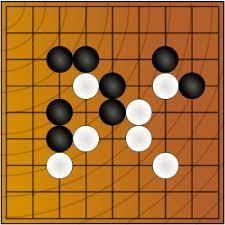
\includegraphics[width=0.9\linewidth,height=0.34\textheight,keepaspectratio]{images/rl-real-world/figures/go.jpg}\\
{\scriptsize \textbf{AlphaGo / AlphaZero}\\(Silver et al.)}
\end{column}
\begin{column}{0.33\textwidth}
\centering
{\scriptsize\textbf{AlphaStar}\\StarCraft II\\(Vinyals et al., 2019)}\\[0.5em]
{\scriptsize\textbf{OpenAI Five}\\Dota 2 (2019)}
\end{column}
\begin{column}{0.33\textwidth}
\centering
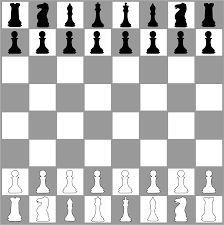
\includegraphics[width=0.9\linewidth,height=0.34\textheight,keepaspectratio]{images/rl-real-world/figures/chess.jpg}\\
{\scriptsize \textbf{Chess} (AlphaZero)}
\end{column}
\end{columns}
\vfill
{\footnotesize \empr{Seen in Part I:} the hide-and-seek agents learned to use tools
the same way, from an automatic curriculum of ever-better opponents.}
\end{frame}
